
% !TeX root = Report.tex
\phantomsection
\addcontentsline{toc}{subsection}{Lecture 3 - Dr Peter Hatto, Head of Research and Development at Ionbond}
\subsect{Lecture 3 - Dr Peter Hatto, Head of Research and Development at Ionbond}

Along with Dr Peter Hatto's role at Ionbond he has previously chaired multiple technical committees on the subject of nanotechnology standardisation.
These include committees \emph{ISO/TC 229}, \emph{CEN/TC 352} and \emph{BSI/NTI/1} preparing such standards as \emph{ISO 10808:2010 Nanotechnologies -- Characterization of nanoparticles in inhalation exposure chambers for inhalation toxicity testing} (section~\ref{sec:lect3})~\cite{iso10808}.
An International Standardisation Organisation (ISO) Technical Committee (TC) is structured, similarly to most ISO/TC, with a chairman coordinating many Working Groups (WGs) followed by Task Groups(TGs).
Figure~\ref{figure:tc229} describes the hierarchy of ISO/TC 229. 

\begin{figure}[!h]
\centering
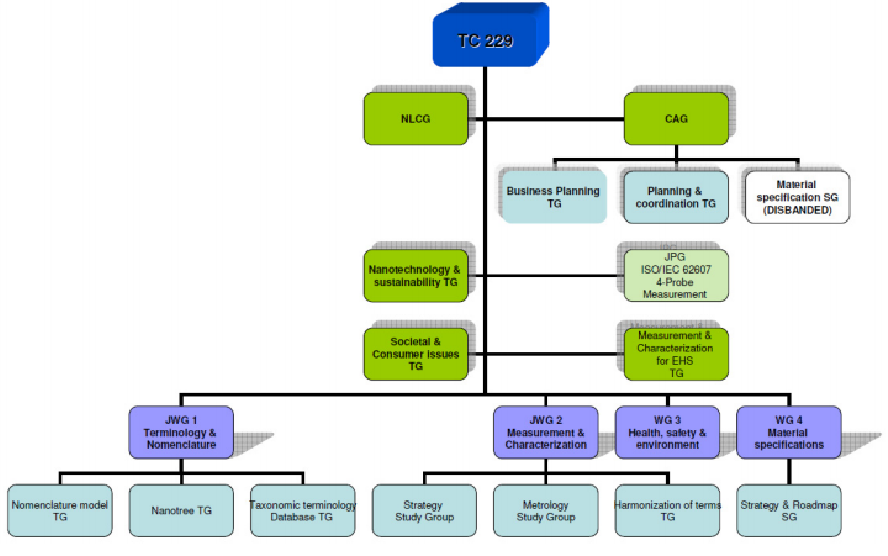
\includegraphics[width = 0.9\textwidth]{Figures/TC229.pdf}
\caption{ISO/TC 229 Structure \cite{isotc229}}
\label{figure:tc229}
\end{figure}

Standards enable modern living by seamlessly allowing not only advanced technology enterprises to work within common space but also basic conformity like \emph{ISO 9407} regarding shoe sizes.
These are a set of rules that can be opted into by businesses then agree to conform to said standard, they are not imposed like regulations.
Agreeing to standardisation can be a catalyst for technological development but also a resistive force if ill-posed.  
This involves controlling four areas of the specific design:

\begin{itemize}
	\item Interoperability
	\item Quality
	\item Variety reduction/optimisation
	\item Information/measurement
\end{itemize}
